\chapter{Event Reconstruction}

The data stored directly from the CMS detector readout contains only the most basic level of information of a collision. As the particles created in the event pass through the detector they create signals at each point they interact, and these signals are locally reconstructed a s a series of ``hits". This raw data is stored in CMS as the data format RAW. In order to undertake physics analyses the information is needed in terms of the four-vectors of particles. In order to interpret the raw data in terms of these physics objects a computational process known as object reconstruction is applied to the data. Using knowledge of the behaviour of each type of object and understanding of the detector, the objects are built from the hits, in such a way that optimises the efficiency for each type of object. Varying sets of requirements called ``identification" or ID can then be applied to these objects at the analyses level to achieve the level of purity required. 

The reconstruction of physics objects happens both within a sub-detector, and also by combining information from two or more sub detectors. The reconstruction is performed under the CMS Software framework (CMSSW) and the reconstructed data is stored in RECO format for use by individual analyses. The main focus of the analysis in this thesis requires well constructed jets and \met, while electron, muon and photon objects are also required for vetoes and control samples. 

\section{Beamspot}

The beamspot represents the locus of the region of beam collision in the detector, where the two bunches of protons meet. It is not an event-by-event measurement, but rather a property of a given physics run, measured over time. It is an important component of reconstruction, as it is used an estimate of the primary vertex, which is the position a given pair of  protons interact to produce an event.

 If the beamspot was at the origin of the CMS detector one would expect the distribution of the track closest approach angle $\phi_{0}$ to be flat in the transverse impact parameter $d_{xy}$. If the beamspot is displaced this behaviour disappears, and thus for each run a fit is made on all available reconstructed tracks to regain this flat behaviour by adjusting the point that $d_{xy}$ is with respect to, yielding the true beamspot. 
 
 
\section{Tracks}

Whilst not a physics object in its own right, one of the most important elements of object reconstructions involves the identification of tracks left by charged particles in the inner tracker. There can then be used along with other sub detectors when reconstructing charged physics objects. In addition these tracks allow a precision identification of the vertex of interaction. In CMS an algorithm called the Combinatorial Track Finder (CTF) is used to construct tracks from their representative hits. 

The reconstruction of a track starts with the construction of a ``seed", an initial candidate track. It contains only a small subset of the available information from the tracker, but must be made up of at least 3 hits, or two hits and an additional beam constraint. The seed represents the initial estimate of the track's trajectory, from which to collect its additional hits. 

In order to achieve the best possible estimate, the seed is built from hits in the innermost area of the tracker, for three important reasons. Although in general the average occupancy decreases with r, the high-density nature of the pixel detector ensures the inner layer of pixel detectors has an occupancy lower than that of the outermost strip detectors. In addition, the pixel detectors give a better estimate of the trajectory due to their truly 2D measurements, and constructing them in the innermost layer minimises the material budget encountered, as not all particles will reach the outer layers. 

The next element of CTF is a patter recognition module based on a Kalman Filter, that proceeds from the seed outwards and includes any additional hits associated with the basic estimated trajectory. As each new measurement is incorporated to the track the trajectory becomes more accurate. This proceeds for each track candidate in parallel, and where several hits are compatible several new candidates are created. 

In order to safeguard against reconstructing one particle as more than one track, an ambiguity resolution mechanism is needed. Given any pair of track-candidates, the fraction of shared hits in the candidate with the fewest hits is examined, and if found to be greater than 50$\%$ this track is removed. If the number of hits is identical then that of the lower $\chi^{2}$ remains while the other is removed. 

Once all compatible hits have been incorporated the most accurate value of the track parameters can be extracted using a final fit. At this point any hits assigned to the track but otherwise not compatible with the track, based on the $\chi^{2}$ of the expected residual, are deemed outliers and discarded before refitting. From the tracks selected, many will be fakes, known as ``ghost" tracks, removed through a set of criteria based upon quality of fit ($\chi^{2}$), the transverse and longitudinal impact parameters $d_{0}$ and $d_{z}$ and the compatibility of the track with what is identified as the interaction vertex. 

The fully CTF algorithm is used iteratively, starting with a pool of all hits identified in that event. After one iteration those hits that have been assigned to a track are removed from the pool, successful tracks are stored, and the process continues with the remaining hits. This process has 6 iterations, decided by the type of seed built. The first two are three-pixel seed and two-pixel seeds respectively, and pick up the high $p_{T}$ tracks of an event. The second and third are also three and two pixel seeds, but with quality criterial loosened as most of the hits have been taken previously. The fifth and sixth iterations allow a seed to be built from strip detectors to include treks which are not covered by the pixel volume.

\section{Vertex}

The exact location of the initial p-p collision of a given event is not necessarily the same as the beamspot (although this cane used as a reasonable estimate) due to the unknown location of a given proton within the bunch . Known as the ``primary interaction vertex", this is reconstructed using the track collection. Selecting prompt tracks based on quality criteria and clustering them in $z$, an adaptive vertex fit is used, where each track receives a weight between 0 and 1 due to its compatability to the vertex common to the set of tracks. 


\section{Jets}
 The QCD property of confinement makes the treatment of partons in collider physics more complicated, as they hadronise once created and are not identified singularly. Additionally these primary hadrons can both emit gluons and decay and fragment into lighter hadrons. These decay products are all travelling in the same direction, as they have been ``boosted" by the momentum of the primary hadron, so each of these groups of particles is called a ``jet". Physics analyses then make requirements on these jets, as opposed to specific requirement of quarks and gluons, where the ``jet" concept in a perfect detector should represent the four-vector of the primary hadron. This is achieved through jet reconstruction where all information left in the detector from the decay products are assigned and added to a jet. As the products are moving under the same boost the jet can be thought to have a cone shape extending from the interaction vertex, where the radius of the cone is defined in the $\eta-\phi$ plane, $R= sqrt{\Delta \eta^{2} + \Delta \phi^{2}}$
 
 At a hadron collider such as the LHC hadronic processes are abundant, and thus the method of defining and reconstructing these jets is crucial to and physics analyses. In CMS there are types of reconstructed jets available, based on the sub-detectors used: Calomieter Jets (CaloJets) use only the ECAL and HCAL, Jet Plus Tracks (JPT) Jets include also information from the tracker, and Particle Flow (PF) Jets use information from the whole detector whilst reconstructing all particles in parallel. The analysis in this thesis uses CaloJets, the reconstruction of which is discussed in more detail below. 
 
 The purpose of jet reconstruction is to group a set of boosted particles together, achieved by an algorithm that "clusters" the information from the calorimeters. The energy deposited in ECAL and HCAL cells are first combined into what are known as ``calorimeter towers", consisting of one or more HCAL cells combined with the ECAL cells which geographically align to the HCAL cell. The tower energy is defined by the sum of cell energies passing an energy threshold to protect against electronic noise. Towers that fulfil the requirement of $E_{T} > 0.3 GeV$ then form the input to the clustering algorithm used by CMS, anti-k$_{T}$~\cite{jetroundup}.

\subsection{The anti-k$_{T}$ jet clustering method}

Due to the expected levels of hadronic activity at the LHC, the jet clustering algorithm must be fast. In addition, it must be stable against the addition of soft particles, called ``infra-red safe", as partons may emit soft gluons. It must also be ``collinear safe", meaning it yields the same jets if a parton were to split into two collinear partons, so that they would both end up in the same jet. These two conditions are essential so that the experimental data may be compared to theoretical calculations regardless of the order they are performed at. 

The anti-k$_{T}$ clustering method \cite{akt} is a sequential recombination algorithm that fulfils these criteria \cite{aktrecom}, working pair-wise to combine nearby towers starting with those highest in $p_{T}$  first. The decision of which order to combine pairs in is achieved with the use of two distance metrics, the distance $d_{ij}$ between two towers $i$ and $j$, and the distance $d_{iB}$ between the $i$th tower and the beam. Considering all possible combinations of both metrics, the smallest is identified. 

If this smallest value is the first case, the two towers i and j are combined into one prototype jet, whose position is weighted by the momenta of its parts. If it is the second case, the tower i is identified as a jet and removed from the list. This process is continued with the updated towers and prototype jets, until all towers have been combined. The definition of the metrics are seen in Equations \ref{eqn:dm1} and \ref{eqn:dm2} where $\Delta_{ij}^{2} = (y_{i}-y_{j})^{2} + (\phi_{i}-\phi_{j})^{2}$. 

 \begin{equation}
d_{ij} = min(k_{ti}^{2p},k_{tj}^{2p})\frac{\Delta_{ij}^{2}}{R^{2}}
\label{eqn:dm1}
\end{equation}
\begin{equation}
d_{iB} = k_{ti}^{2p}
\label{eqn:dm2}
\end{equation}

Tower $i$ has transverse momentum $k_{ti}$, rapidity $y_{i}$ and azimuth $\phi_{i}$. The variable R is analogous to the cone radius definition described above, and for this analysis R = 0.5. This general form of the metrics governs several types of jet algorithm of this family, differing in the value of power $p$. This is the parameter responsible for the relative importance of momenta and distance, and for anti-k$_{T}$ p = -1 placing the importance on the momenta, and giving the ``anti" in its name (after another variant, the k$_{T}$ algorithm for which p = +1~\cite{kt}).

In this algorithm a hard particle creating a large energy deposit with no other hard deposits surrounding it will gather in the soft particle deposits. If another hard particle is found within 2R then the soft deposits are shared between them with weights relative to the hard particle momenta, unless they are within R of one another in which case they are identified as one jet. 

The shape of the jet is defined alone by the cone about the hard particle, resulting in a perfectly conical jet except in the case where more than one hard particle exists within 2R. If the two hard jets are within R or one another, the shape is either dominated by the hardest if there is a significant difference in the momenta, or if they are similar, defined by the total area covered by both cones. If the jets are not within R but within 2R, there is not space for each jet to be conical, so either the hardest jet is conical and the softer is missing a piece, or if they have similar momenta each has a chunk missing with a boundary line down the middle of the shared area. Figure \ref{fig:akt} shows in the y-$\phi$ plane jets reconstructed by anti-k$_{T}$ for a sample event (generated by Herwig) in which many soft deposits exist. Many coloured circular jet patterns are seen, representing conical jets, as well as the cases with close hard deposits demonstrating the shared and clipped jet area shapes. 

\begin{figure}
\centering
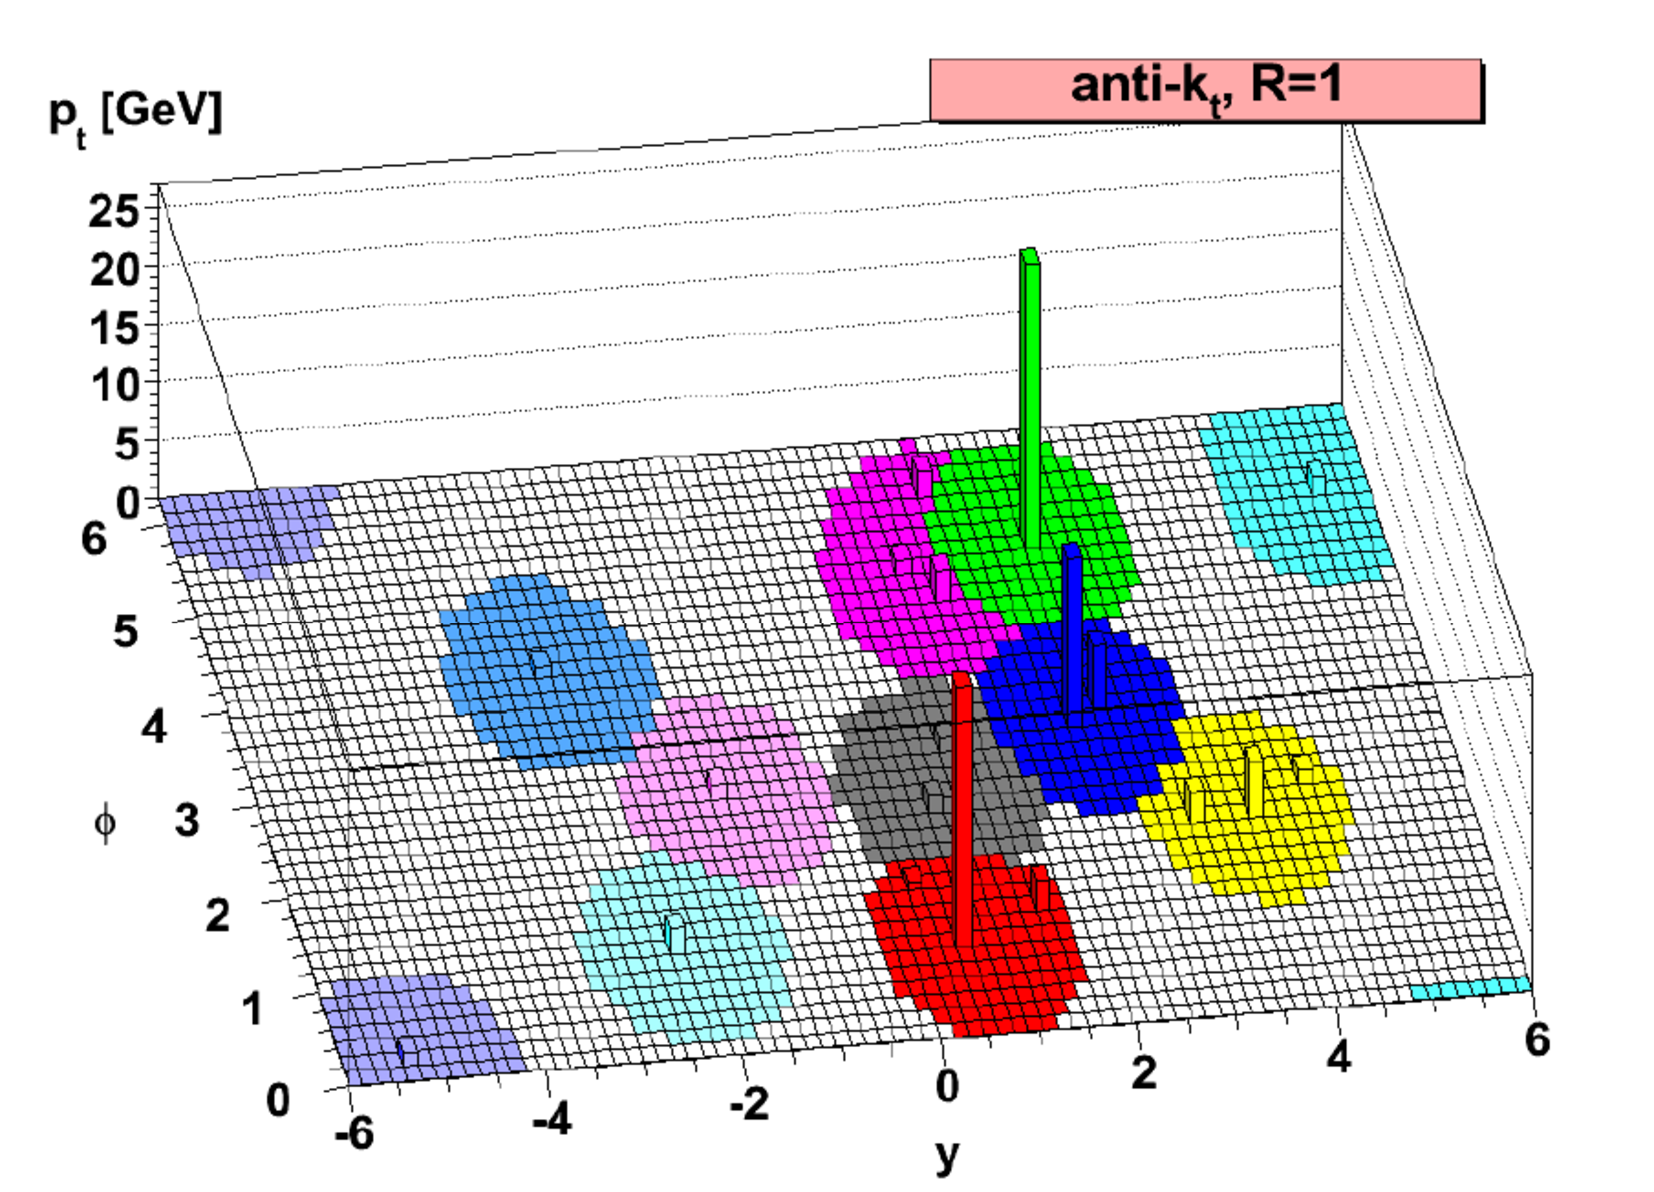
\includegraphics[width=0.7\textwidth]{Figures/Objects/akt}
\caption{\label{fig:act}Illustration of the reconstructed jets for a sample Herwig generated event, with many soft deposits. Each coloured area represents the shape of the jet reconstructed, illustrating the trend to a conical nature of anti-k$_{T}$, and the behaviour of the algorithm where two hard deposits are close. Taken from \cite{akt}.}
\end{figure}

Contamination from both pileup and underlying events can contribute soft energy deposits which may affect the momenta of jets reconstructed, the effect of which is known as the ``back reaction". One of the major advantages of the anti-k$_{T}$ algorithm is that due to the relative importance of hard deposits over softer deposits this effect is suppressed, allowing more accurate measurement of jet momenta than other comparable models, leading to its selection by CMS.
\subsection{Jet Energy Scale Corrections}

The jets reconstructed in the detector using the method above typically have an energy that is different to that we would measure in a perfect situation. This is due to the nature of the response of the calorimeters, which is non-linear and non-uniform, as well as any residual effect contributed from pileup and underlying events (although this is small as mentioned above). For this reason, reconstructed jets must undergo energy corrections before they can be used in physics analyses. 

The aim of these Jet Energy Scale (JES) corrections is to relate the energy measured in the detector to the energy of the underlying jet particles through knowledge of the detector response. This is achievied by the following three levels of correction 

\begin{description}
\item[L1 - Offset]{An offset is subtracted to remove the energy contributions that are not associated with the event but rather from electronic noise and pileup events.  }
\item[L2 - Relative]{Next the value is multiplied by a factor which is a function of a given pseudorapidity $\eta$ to correct the relative differences in repines in different regions of the calorimeters.}
\item [L3 - Absolute]{Finally the value is multiplied by a second factor, which corrects the variable response to different jet p$_{T}$. The response to a given particle never returns the entire proportion of energy, and the percentage returned depends heavily on the momenta of the particle.}
\end{description}



Initially an estimate of the correction is calculated with the help of Monte Carlo truth information, representing the major portion of the calibration. Here instead of separating the three levels, an all-together approach is used. Events generated by \textsc{PYTHIA} are passed through the full CMS detector simulation \textsc{GEANT 4}, in order to identify the reconstructed jets. In addition, full information for the real physical jets, \textit{generator} jets is retained. Each reconstructed jet is matched its own generator jet in the $\eta - \phi$ plane, making a requirement on the cone radius R < 0.25 to avoid mis-matching. A comparison of the momenta of the reconstructed jet and the generator jet allows a calibration factor to be extracted relative to the jet's $\eta$ and $\phi$. 

Having calibrated the momenta using Monte-Carlo data-driven corrections of the relative and absolute calibrations are made. The relative correction is extracted using di-jet events balanced in $p_{T}$ where one is detected in the central region, and the other may have any $\eta$ value. The measurement of the second jet energy is compared to the well-defined measurement of the central region (chosen as the control region as it delivers the best performance for high p$_{T}$ jets) in order to return the correction factor dependant on $\eta$.  Having applied this correction, another is performed for the absolute using an events where a photon lies back to back with a jet. Comparing the momenta of the two gives an understanding of the distribution of the percentage of energy that has been included in a jet yielding the required factor.

With the application of the three levels of correction, the total energy of the particles within the jet has been recovered to an acceptable level required by the physics analyses of CMS. The jet used in this analysis correspond to a calibration with precision corresponding to an $3 - 6 \%$ uncertainty of the jet energy scale (JES) for jet momenta ranging from 30 GeV up to 2TeV~\cite{JME_10_010}.

\section{Missing Energy}

As previously mentioned the LSP if it exists would not react, meaning its typical signature in a detector is that of energy gone undetected. This is observed as a momentum imbalance, or ``missing energy" of the observed particles, the transverse component of which is the preferred search variable, \met. 


\section{Electrons}

\section{Muon}
